\section{Results}
\label{sec:results}

\subsection{Fixed Cutoffs Alter Measured Effects}

Figure~\ref{fig:fixed-l-diagnostics} compares DESA with Original at $L=50$ and
under complete-list fusion. Each query--draw pair is a gain, tie, or loss;
off-diagonal cells mark a changed judgment.

\begin{figure}[H]
\centering
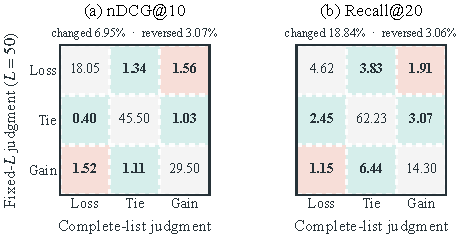
\includegraphics[width=\columnwidth]{figures/fig_fixed_top_l_diagnostics.pdf}
\caption{Transition between the DESA-versus-Original judgment at fixed
$L=50$ (rows) and under complete-list fusion (columns). Cells report the
equal-dataset percentage of query--draw pairs. Green off-diagonal cells change
among gain, tie, and loss; red cells are strict gain--loss reversals.}
\label{fig:fixed-l-diagnostics}
\end{figure}

At $L=50$, 6.95\% of nDCG judgments and 18.84\% of Recall judgments differ
from complete-list fusion. Strict gain--loss reversals account for 3.07\% and
3.06\%, respectively. Other cutoffs and ordered top-20 agreement appear in
Appendix Table~\ref{tab:cutoff-query-diagnostics}.

\subsection{Complete-List Effectiveness and Certification Depth}

Table~\ref{tab:main-results} reports the primary complete-list comparison.
DESA reaches .4747 nDCG@10 and .4695 Recall@20, gains of 3.82\% and 2.38\%
over Original. Dense and sparse certification depths fall by 36.90\% and
36.56\%, and 63.31\% of queries become shallower in both channels. All four
differences remain significant after Holm correction
($p_{\mathrm{Holm}}=.0004$).

\begin{table}[H]
\centering
\scriptsize
\setlength{\tabcolsep}{3.2pt}
\begin{tabular}{lrrrr}
\toprule
Method & nDCG@10 $\uparrow$ & Recall@20 $\uparrow$ & $L_D\downarrow$ & $L_S\downarrow$ \\
\midrule
\multicolumn{5}{l}{\textit{Original query}} \\
Original & 0.4572 & 0.4586 & 1752.4 & 1455.1 \\
\addlinespace[1pt]
\multicolumn{5}{l}{\textit{Shared expansion}} \\
Shared & 0.4671 & 0.4666 & \textbf{607.4} & \textbf{606.7} \\
\addlinespace[1pt]
\multicolumn{5}{l}{\textit{Single-channel construction}} \\
Dense only  & 0.4621 & 0.4637 & 1386.5 & 1219.9 \\
Sparse only & \underline{0.4714} & \underline{0.4678} & 884.4 & 822.0 \\
\addlinespace[1pt]
\multicolumn{5}{l}{\textit{Channel-asymmetric construction}} \\
DESA & \textbf{0.4747} & \textbf{0.4695} & \underline{728.9} & \underline{673.2} \\
\bottomrule
\end{tabular}
\caption{Equal-dataset macro results for the seven-dataset controlled
comparison. Higher is better for retrieval metrics; lower is better for replay
stopping depths. Raw depths are averaged across datasets; percentage reductions
in the text are computed within each dataset before macro-averaging.}
\label{tab:main-results}
\end{table}

Shared expansion reaches lower raw depths but also lower nDCG. Because it uses
the same references as DESA, the difference isolates how shared evidence is
integrated across channels.

\subsection{Cross-Channel Coordination}

The matched Shared comparison isolates integration while holding generated
evidence fixed. DESA improves macro nDCG by 1.61\% and Recall by 0.61\%.
The nDCG difference is significant ($+.0075$;
$p_{\mathrm{Holm}}=.0012$), whereas Recall ($+.0028$;
$p_{\mathrm{Holm}}=.2736$) and both depth differences are not. The evidence
therefore supports a quality benefit from coordinated integration, but not a
depth advantage over Shared.

The sparse channel shows why shared evidence requires coordinated integration.
Shared expansion enlarges sparse support on six datasets, by as much as
$5.72\times$. On NFCorpus, support grows from 561.5 to 3211.6 documents and
sparse depth rises by 105.81\%. DESA instead preserves virtually all Original
support while reducing sparse and dense depth by 23.15\% and 15.03\%.
Table~\ref{tab:channel-evidence} extends this contrast across datasets.

\begingroup
\definecolor{effhead}{HTML}{DCEFEA}
\definecolor{accesshead}{HTML}{E2E7F5}
\definecolor{supporthead}{HTML}{FAEDC9}
\definecolor{positive}{HTML}{E7F5F0}
\definecolor{negative}{HTML}{F3D4CE}
\definecolor{access}{HTML}{EBEEF9}
\definecolor{broaden}{HTML}{FFF2CF}
\definecolor{preserve}{HTML}{DDF2E9}
\definecolor{pattern}{HTML}{EEF0F2}
\newcommand{\effcell}[1]{\colorbox{positive}{\strut\makebox[3.25em][c]{#1}}}
\newcommand{\negcell}[1]{\colorbox{negative}{\strut\makebox[3.25em][c]{\textbf{#1}}}}
\newcommand{\accesscell}[1]{\colorbox{access}{\strut\makebox[3.25em][c]{#1}}}
\newcommand{\broadcell}[1]{\colorbox{broaden}{\strut\makebox[3.65em][c]{#1}}}
\newcommand{\keepcell}[1]{\colorbox{preserve}{\strut\makebox[3.65em][c]{#1}}}
\newcommand{\patterncell}[1]{\colorbox{pattern}{\strut\scriptsize\textbf{#1}}}
\begin{table*}[t!]
\centering
\scriptsize
\setlength{\tabcolsep}{3.0pt}
\renewcommand{\arraystretch}{1.20}
\begin{tabular}{lrrrrrrr}
\toprule
& \multicolumn{3}{c}{\colorbox{effhead}{\strut\textbf{Effectiveness: relative $\Delta$nDCG@10 (\%)}}}
& \multicolumn{2}{c}{\colorbox{accesshead}{\strut\textbf{Replay-depth reduction (\%)}}}
& \multicolumn{2}{c}{\colorbox{supporthead}{\strut\textbf{Sparse support ($\times$ Original)}}} \\
\cmidrule(lr){2-4}\cmidrule(lr){5-6}\cmidrule(lr){7-8}
\textbf{Dataset}
& \textbf{DESA vs. Orig.}
& \textbf{+Dense given Sparse}
& \textbf{+Sparse given Dense}
& $\boldsymbol{L_D}$
& $\boldsymbol{L_S}$
& \textbf{Shared}
& \textbf{DESA} \\
\midrule
SciFact
& \effcell{+2.40} & \effcell{+1.12} & \effcell{+0.91}
& \accesscell{22.2} & \accesscell{20.9}
& \broadcell{1.62$\times$} & \keepcell{1.00$\times$} \\
NFCorpus
& \effcell{+3.37} & \effcell{+2.14} & \effcell{+1.36}
& \accesscell{15.0} & \accesscell{23.2}
& \broadcell{\textbf{5.72$\times$}} & \keepcell{1.00$\times$} \\
TREC-COVID
& \effcell{+5.69} & \effcell{+0.51} & \effcell{+4.68}
& \accesscell{74.9} & \accesscell{66.7}
& \broadcell{1.53$\times$} & \keepcell{1.00$\times$} \\
FiQA
& \effcell{+3.61} & \negcell{$-$0.66} & \effcell{+3.74}
& \accesscell{49.7} & \accesscell{48.7}
& \broadcell{1.64$\times$} & \keepcell{1.00$\times$} \\
ArguAna
& \effcell{+1.27} & \effcell{+0.32} & \effcell{+0.88}
& \accesscell{15.2} & \accesscell{15.3}
& \broadcell{1.00$\times$} & \keepcell{1.00$\times$} \\
Touch\'e-2020
& \effcell{+7.52} & \effcell{+0.92} & \effcell{+5.70}
& \accesscell{45.8} & \accesscell{45.8}
& \broadcell{1.88$\times$} & \keepcell{1.00$\times$} \\
SCIDOCS
& \effcell{+0.86} & \effcell{+0.03} & \effcell{+0.13}
& \accesscell{35.4} & \accesscell{35.4}
& \broadcell{2.02$\times$} & \keepcell{1.00$\times$} \\
\midrule
\textbf{Pattern}
& \patterncell{7/7 improve}
& \patterncell{6/7 improve}
& \patterncell{7/7 improve}
& \patterncell{7/7 shallower}
& \patterncell{7/7 shallower}
& \patterncell{up to 5.72$\times$}
& \patterncell{$\approx$1.00$\times$} \\
\bottomrule
\end{tabular}
\caption{Per-dataset evidence for cross-channel coordination.
Effectiveness columns report relative nDCG@10 changes; +Dense and +Sparse
compare DESA with the corresponding one-operator construction. Depth columns
report replay stopping-depth reductions from Original, where positive values
indicate smaller certified prefixes. Sparse support is normalized by Original;
red marks the sole degradation.}
\label{tab:channel-evidence}
\end{table*}
\endgroup

The $2\times2$ comparison reveals unequal but complementary roles. Dense
expansion alone improves nDCG and Recall by 1.08\% and 1.11\%, with dense and
sparse depth reductions of 8.16\% and 7.49\%. Sparse anchoring yields gains of
3.11\% and 2.01\%, with reductions of 28.77\% and 27.74\%. Adding Sparse
anchoring to Dense only improves nDCG on all seven datasets; adding Dense
expansion to Sparse only improves six, with FiQA at $-0.66\%$. Their
combination nevertheless improves over Original and reduces both depths on
every dataset.

The matched operator controls sharpen this conclusion. Residual dense expansion
does not significantly outperform unprojected expansion, nor does score-product
anchoring significantly outperform direct sparse rewriting. Yet full DESA
improves Original on every dataset and significantly improves nDCG over Shared.
The consistent advantage therefore belongs to the coordinated construction,
not to a demonstrably superior isolated operator. Sparse-support preservation
is exact on six datasets and 99.9999\% on Touch\'e-2020, whose exported tail
omits 25 extremely low-scoring document occurrences. Angle, turnover, rank-movement,
binary-mask, reference-count, and operator-control diagnostics appear in
Appendices~\ref{sec:appendix-mechanism} and~\ref{sec:appendix-analysis}.

\subsection{Comparison with Expansion and Fusion Methods}

Table~\ref{tab:fidelity} compares DESA with matched QuDAR and reproduced
expansion methods. Under matched references, QuDAR and DESA achieve similar
complete-list effectiveness; neither paired metric difference is significant.
DESA reduces total certification depth by 74.41\% (95\% CI: 67.27--80.89;
$p_{\mathrm{Holm}}=.0002$).

\begin{table}[H]
\centering
\scriptsize
\setlength{\tabcolsep}{2.4pt}
\begin{tabular}{lrrr}
\toprule
Method & nDCG@10 $\uparrow$ & Recall@20 $\uparrow$ & Total depth $\downarrow$ \\
\midrule
\multicolumn{4}{l}{\textit{Matched references, seven datasets}} \\
QuDAR-complete & \textbf{0.4760} & \textbf{0.4712} & \underline{5478.4} \\
DESA         & \underline{0.4747} & \underline{0.4695} & \textbf{1402.1} \\
\addlinespace[1pt]
\multicolumn{4}{l}{\textit{Prior query expansion, seven datasets}} \\
Original     & 0.4572 & 0.4586 & 3207.6 \\
HyDE         & 0.4114 & 0.4374 & 16668.8 \\
MuGI         & 0.4584 & 0.4596 & 2790.1 \\
Query2doc    & \underline{0.4728} & \underline{0.4675} & \underline{1771.5} \\
DESA         & \textbf{0.4747} & \textbf{0.4695} & \textbf{1402.1} \\
\bottomrule
\end{tabular}
\caption{External comparisons over the same seven evaluation datasets. Total
depth sums the policy-specific replay depths of all rankings used by each
complete-list fusion target.}
\label{tab:fidelity}
\end{table}

Among reproduced expansion methods, DESA has the highest effectiveness and the
lowest total depth. Its closest baseline, Query2doc, is slightly lower on both
metrics and requires greater total depth. These comparisons are descriptive;
we do not claim paired significance for the lower block of
Table~\ref{tab:fidelity}.

\subsection{Robustness and Failure Boundary}

With Mistral, all four sampled datasets retain non-negative effectiveness
changes. Dense and sparse depth reductions range from 7.12\% to 47.61\% and
7.16\% to 47.62\%; 10\% of sampled ArguAna queries trigger the structured-output
fallback.

With Contriever, both effectiveness metrics improve on all four datasets.
Touch\'e-2020 nevertheless increases dense and sparse depths by 14.29\% and
4.34\%, the only setting where both worsen. TREC-COVID gains remain positive
but non-monotonic across corpus sizes. Appendix~\ref{sec:additional-results}
reports the remaining generator, encoder, reference-count, fusion, and scale
results.

\FloatBarrier
